\section{Selected-tensor results and source-linked robustness}
\label{sec:results}

\subsection{Likelihood values and the signed tensor}

Table~\ref{tab:likelihood} gives the saved residual quadratics, maximum-likelihood scales, and normalized likelihood values. These values refer to the same fifteen-coordinate mean and the same 274 responses. Their consistency with the retained row likelihood was checked independently through the sufficient statistics: the largest absolute log-likelihood discrepancy was $1.1\times10^{-12}$, and the largest scaled covariance discrepancy was $9.1\times10^{-15}$, rounded upward. This verifies the stated arithmetic within numerical precision. It does not test the Gaussian or selection assumptions.

\begin{table}[htb]
\caption{Full-model likelihood summaries on the same 274 released rows. The scale is the dimensionless maximum-likelihood multiplier $q_s/274$. The final column is the smallest two-sided tail among the five predictive $F$ diagnostics for that shape; it is not a combined probability.}
\label{tab:likelihood}
\begin{ruledtabular}
\begin{tabular}{rrrrrr}
$a$ [mag]&$b$ [mag]&$q_s$&$\widehat\sigma^2_{\rm ML}$&$\log L_s(\widehat\beta_s,\widehat\sigma^2_{\rm ML})$&Minimum fold tail\\
0&0&651.218204&2.376709&$-168.298506$&0.109525\\
0&0.29&324.919303&1.185837&$-173.029455$&0.023265\\
0.055&0&682.763995&2.491839&$-170.021994$&0.113920\\
0.055&0.29&330.452668&1.206032&$-173.703843$&0.024920
\end{tabular}
\end{ruledtabular}
\end{table}

The tensor estimates in Table~\ref{tab:stf} retain all five signs. The second component changes substantially with the group-covariance scenario, whereas the fifth is nearly stable. Such componentwise differences cannot be represented by a single amplitude change. Figure~\ref{fig:regions} displays coordinate projections of the full joint regions, with the earlier Gaussian-reference projections retained for comparison. All four projected tensor regions contain the zero tensor: the corresponding historical joint-radius check already contained zero, and the finite-$F$ radius is larger. This conclusion concerns the selected statistical tensor, not the absence of physical anisotropy.

\begin{table}[htb]
\caption{Signed STF coefficient estimates in the basis of Eq.~\eqref{eq:tensorbasis}, in magnitudes. These are five-coordinate views of the joint fifteen-coordinate fits; the complete covariance is retained in the accompanying numerical sources.}
\label{tab:stf}
\begin{ruledtabular}
\begin{tabular}{rrrrrrr}
$a$ [mag]&$b$ [mag]&$\widehat b_1$&$\widehat b_2$&$\widehat b_3$&$\widehat b_4$&$\widehat b_5$\\
0&0&0.183056&0.808292&$-0.010452$&0.045121&0.126844\\
0&0.29&0.195454&0.595818&0.038591&$-0.028036$&0.128076\\
0.055&0&0.180529&0.831115&$-0.017713$&0.048508&0.127592\\
0.055&0.29&0.195170&0.599207&0.037642&$-0.026498$&0.128246
\end{tabular}
\end{ruledtabular}
\end{table}

\begin{figure}[p]
\centering
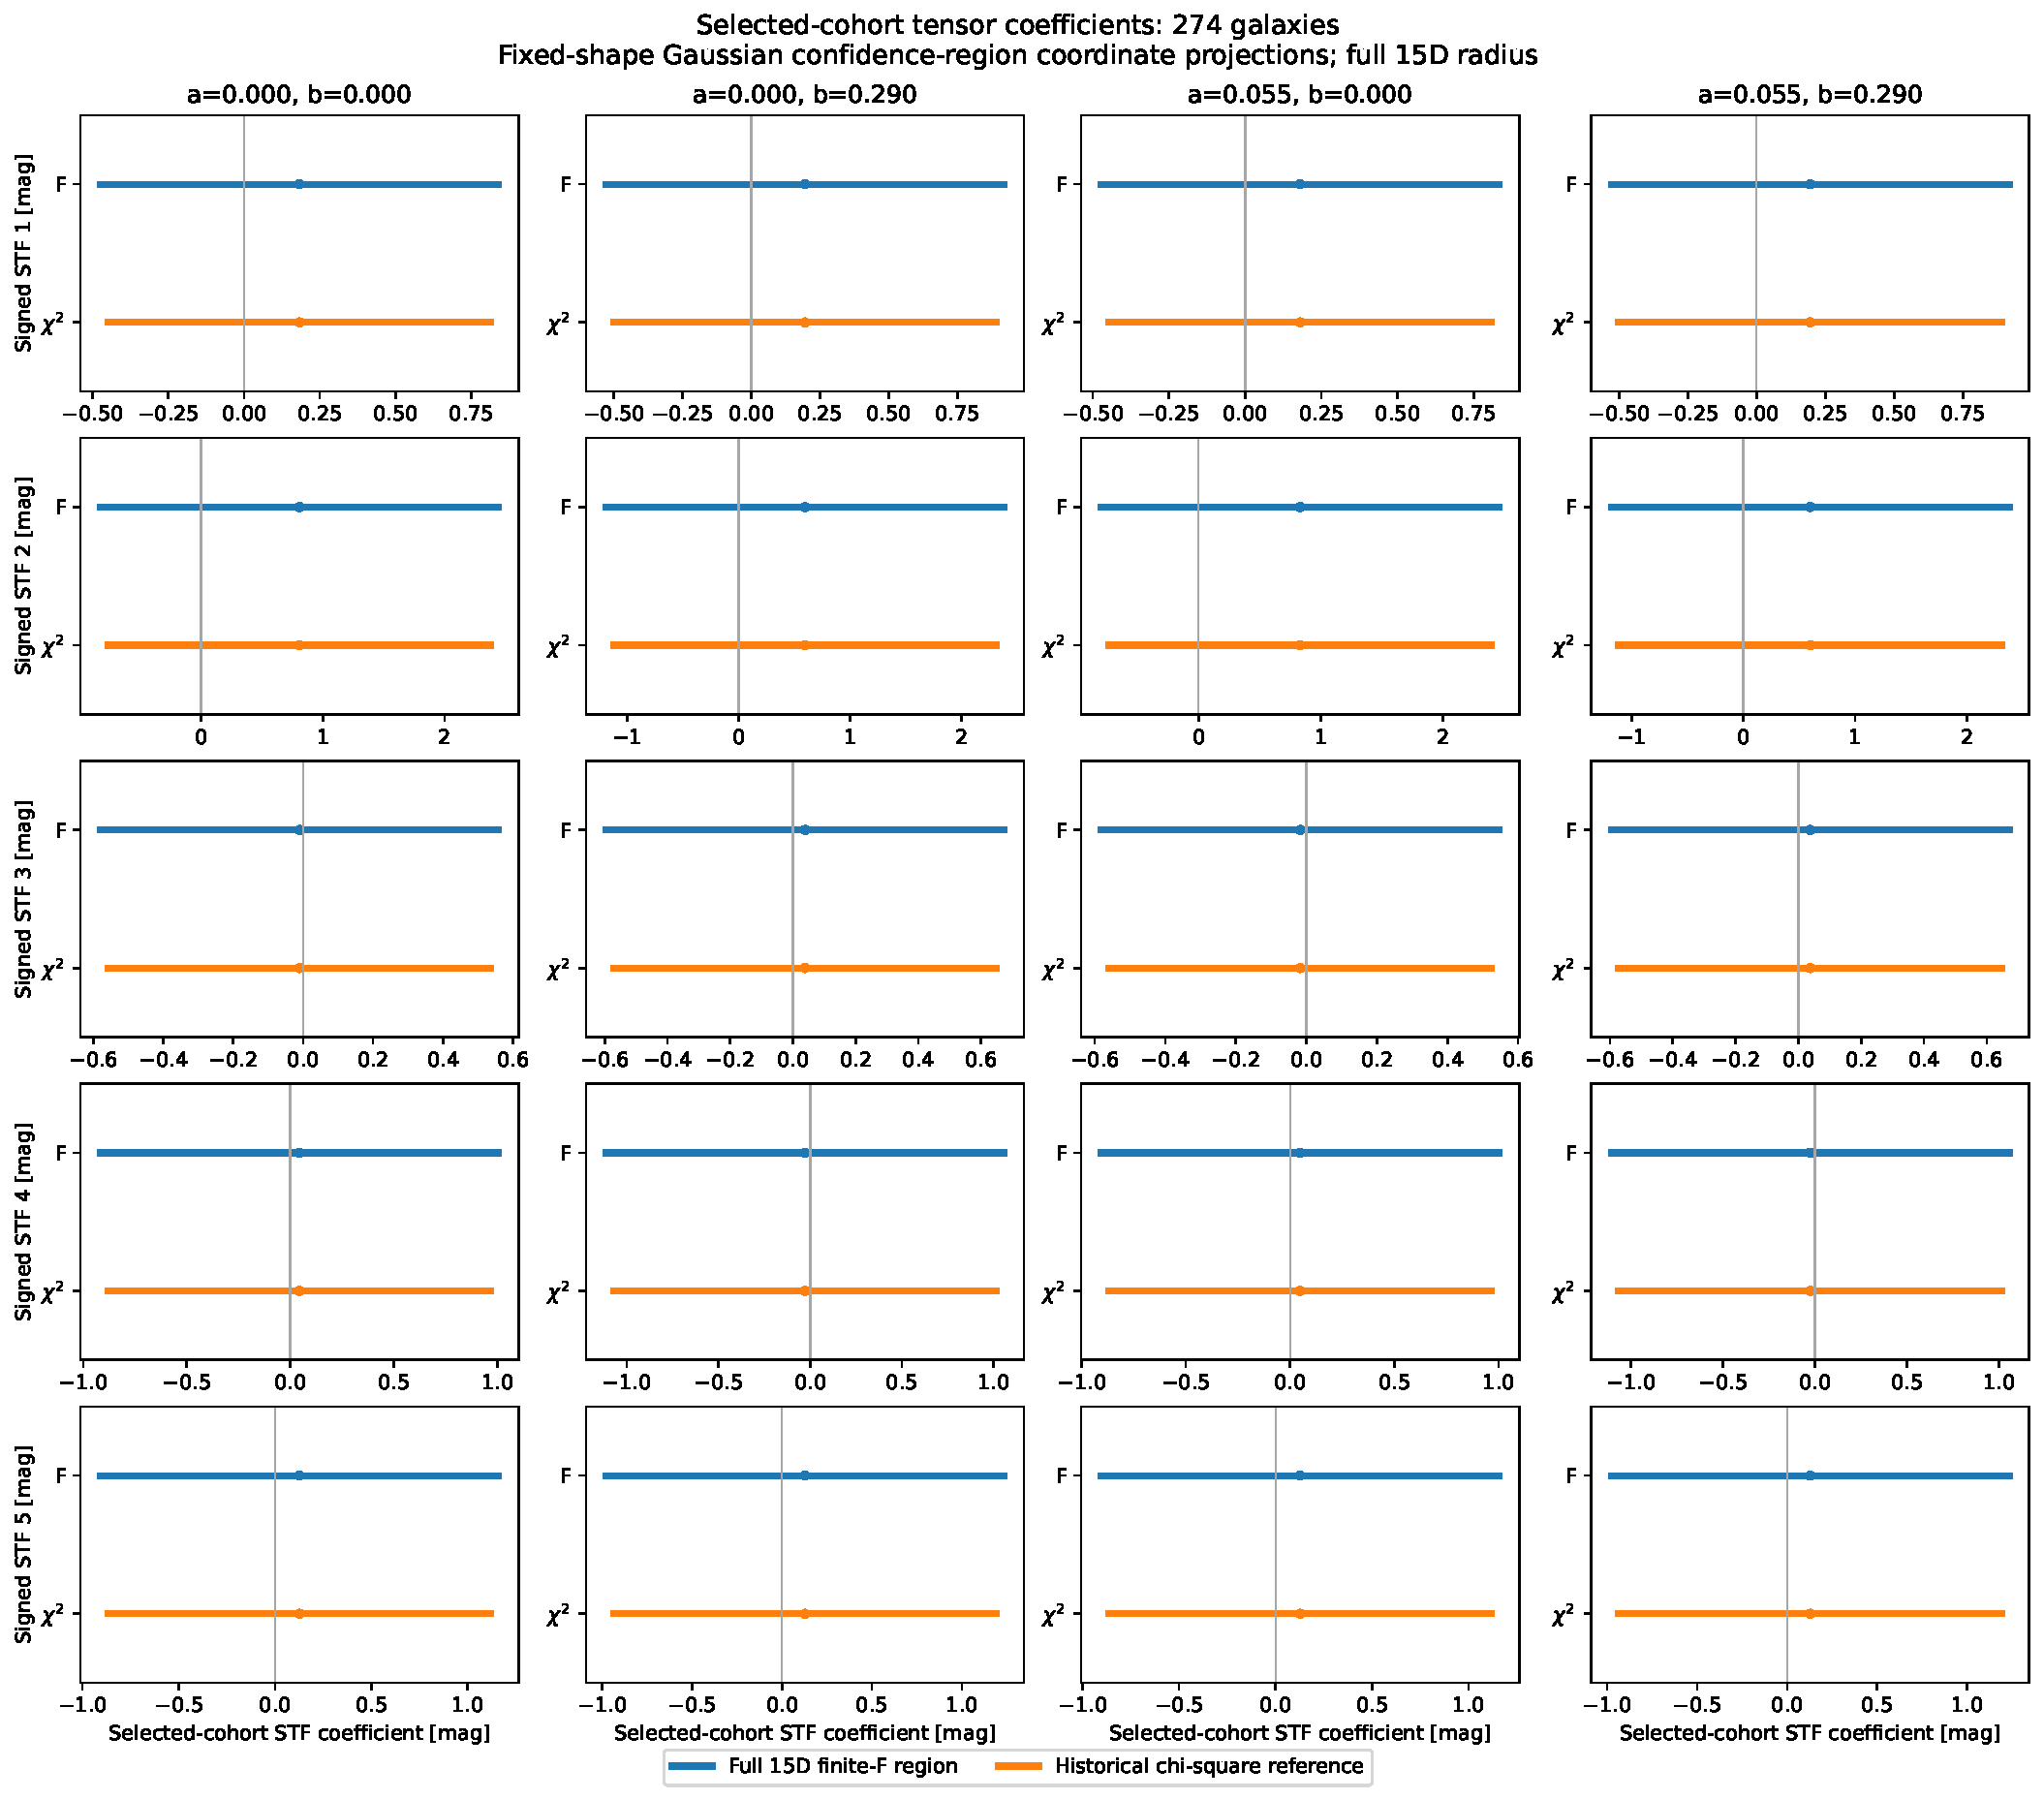
\includegraphics[width=.95\textwidth,height=.76\textheight,keepaspectratio]{figures/selected_tensor_law.pdf}
\caption{Five signed STF coordinates under four covariance shapes. The finite-$F$ intervals are coordinate projections of the full fifteen-parameter model-conditional 95\% region, with all nuisance parameters retained before projection. The historical chi-square intervals are fixed-Gaussian algebraic references, not exact finite-sample regions for an estimated scale. The plotted intervals do not replace the joint tensor covariance and do not give physical shear bounds.}
\label{fig:regions}
\end{figure}

The smallest predictive two-sided tail across all twenty entries is $0.0232647095087$. None crosses $0.0025$. This statement is compatible with poor predictive scores for some models: the two calculations answer different questions. The finite-$F$ check includes training-coefficient uncertainty, whereas the saved scoring rule below uses a plug-in prediction covariance. In addition, a lack of rejection at a conservative retrospective threshold does not demonstrate an adequate physical model.

\subsection{Model comparison changes with group covariance}

We compare three retained mean models on exactly the same rows and whole-group folds. Model A has the four baseline columns, the shared calibration dipole, and the three $K_i n_i$ columns; it has ten coefficients. Model B replaces the latter vector response with five STF columns and has twelve coefficients. Model C includes both responses and has fifteen coefficients, as in Eq.~\eqref{eq:design}. These are competing selected-window mean descriptions, not three identified cosmological geometries.

For each fold the retained score uses the normalized block-conditional Gaussian density with mean in Eq.~\eqref{eq:predictor} and covariance $\widehat\sigma^2_{{\rm ML},t}W_s$. Training-coefficient and scale uncertainty are omitted from this plug-in density. We preserve that procedure rather than retrospectively replacing its scores with a different predictive law. Scores are summed over the five held-out blocks; larger values indicate better prediction for this scoring procedure within one covariance scenario. They are not marginal likelihoods or Bayes factors.

\begin{table}[htb]
\caption{Summed joint held-out log densities on the same 274 responses. Every row uses the same folds. The scores are retrospective plug-in comparisons with training-parameter uncertainty omitted; they are separate from Eq.~\eqref{eq:predf}.}
\label{tab:comparison}
\begin{ruledtabular}
\begin{tabular}{rrrrr}
$a$ [mag]&$b$ [mag]&A: vector response&B: STF response&C: both\\
0&0&$-220.320018$&$-196.843320$&$-518.193732$\\
0&0.29&$-194.273316$&$-195.138036$&$-209.534052$\\
0.055&0&$-231.854820$&$-198.339595$&$-651.993130$\\
0.055&0.29&$-193.723069$&$-194.545441$&$-209.464523$
\end{tabular}
\end{ruledtabular}
\end{table}

The ordering reverses. Model B leads when the added group covariance is zero; model A leads narrowly when $b=0.29\,\mathrm{mag}$. Model C performs poorly, especially without the group term. Hence the retained evidence does not support a covariance-insensitive preference for one angular response. Figure~\ref{fig:models} shows the score dependence together with signed residual summaries. Small aggregated residual means do not remove this instability or certify the residual distribution.

There is also a directly interpretable domain failure. For PGC 9031, with $V_{\rm CMB}=317\,\kms$, the fitted vector contribution in model C corresponds to a flow fraction approximately $2.26$--$2.45$ across the covariance choices. A small-velocity interpretation of Eq.~\eqref{eq:kresponse} is invalid there. The coefficient can remain a term in a phenomenological regression, but interpreting it as a perturbative physical flow would exceed its approximation domain. Removing that object after inspecting the scores would define a new analysis.

An earlier seven-column Gaussian residual candidate on this cohort also failed an actual-data check: its retained discrepancy was $T=4.555321823822732$, with three simulated values at least as extreme among 4096 reference realizations, giving the recorded plus-one rank $4/4097=0.000976324139614352$. This is a failure of that specified working residual candidate. It is not a calibrated test of the later A/B/C alternatives, and repeated simulations from the old candidate cannot repair its observed discrepancy. We retain the failure because model criticism must remain attached to the model and source on which it occurred.

\begin{figure}[p]
\centering
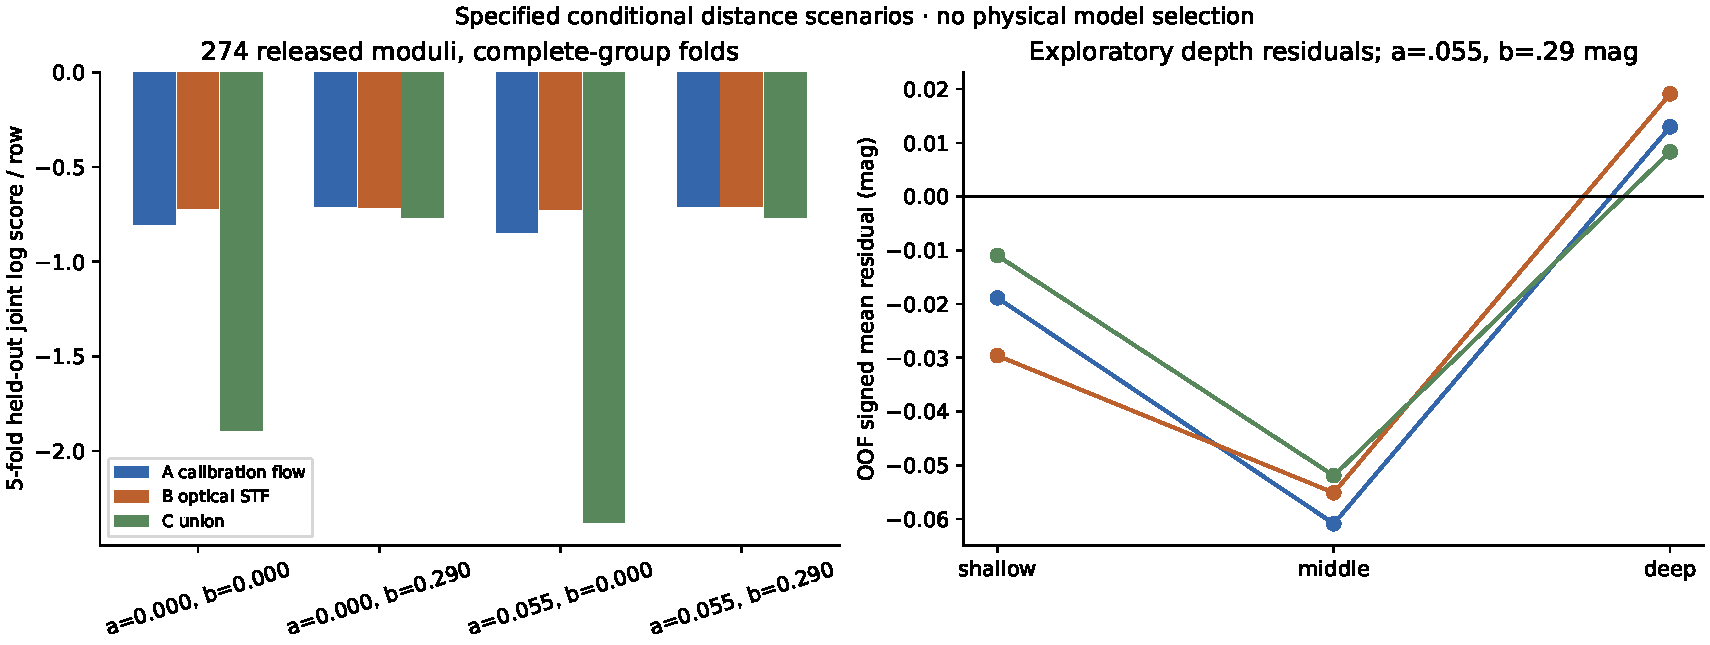
\includegraphics[width=.95\textwidth,height=.76\textheight,keepaspectratio]{figures/model_comparison.pdf}
\caption{Retained whole-group prediction scores and signed residual summaries for the three mean models on the same observed cohort. The ordering of vector and STF models changes with the declared group covariance. These plug-in scores do not include training-coefficient or scale uncertainty and are not the finite-$F$ diagnostics. The fitted angular terms remain selected-window responses.}
\label{fig:models}
\end{figure}

\subsection{Missing outcomes and the target-frame fraction}

For a fixed model and covariance choice, consider the event $|r_i|>t$ for the saved held-out signed residual $r_i$ in magnitudes. At $t=0.5\,\mathrm{mag}$, the count $m$ among the 274 observed objects ranges from 71 to 80 over the twelve retained cases. If the 354 missing event indicators are unrestricted, the exact attainable set of the uniform 628-target fraction is
\begin{equation}
 \mathcal J_m=\left\{\frac{m+k}{628}:k=0,1,\ldots,354\right\}.
 \label{eq:missingframe}
\end{equation}
Its smallest containing interval has width $354/628=0.5636942675$. The set itself is discrete. Reporting the hull does not make every intermediate fraction attainable by a deterministic completion.

We also vary a declared measure on the observed cohort. If its original uniform event mass is $e=m/274$ and the new density ratio lies in $[1/\Gamma,\Gamma]$ with mean one, then the sharp event-mass endpoints are
\begin{align}
 L_\Gamma(e)&=\max\{e/\Gamma,1-\Gamma(1-e)\},\nonumber\\
 U_\Gamma(e)&=\min\{\Gamma e,1-(1-e)/\Gamma\}.
 \label{eq:densitybounds}
\end{align}
The proof uses the constraints on the event and its complement, and constant within-class densities attain the endpoints. This is a normalized density-ratio class; two atomic density ratios may differ by $\Gamma^2$. It is not the different convention that bounds only the ratio between the largest and smallest weights.

Holding the observed target mass fixed at $274/628$, the completed set becomes
\begin{equation}
 \bigcup_{k=0}^{354}\left[
 \frac{274}{628}L_\Gamma(e)+\frac{k}{628},\;
 \frac{274}{628}U_\Gamma(e)+\frac{k}{628}\right].
 \label{eq:completedweighted}
\end{equation}
At $\Gamma=2$ and $t=0.5\,\mathrm{mag}$ its hull widths are $0.7333$--$0.7548$; at $\Gamma=4$ they are approximately $0.8909$. Figure~\ref{fig:selection} retains all model--shape cases rather than selecting a favourable curve. The availability fraction $274/628$ is not an estimated inclusion propensity for a larger population. These are mathematical sensitivity sets for the known finite target frame, not confidence intervals for a physical anisotropy fraction.

For signed means the limitation is stronger. Assigning an arbitrary common residual $R$ to all missing objects changes the target mean by $(354/628)R$. Its range is unbounded in that completion model. This statement requires no probabilistic imputation and does not assert a physically realizable range for a cosmological tensor. A physical support restriction, if justified separately, would change the identified set.

\begin{figure}[p]
\centering
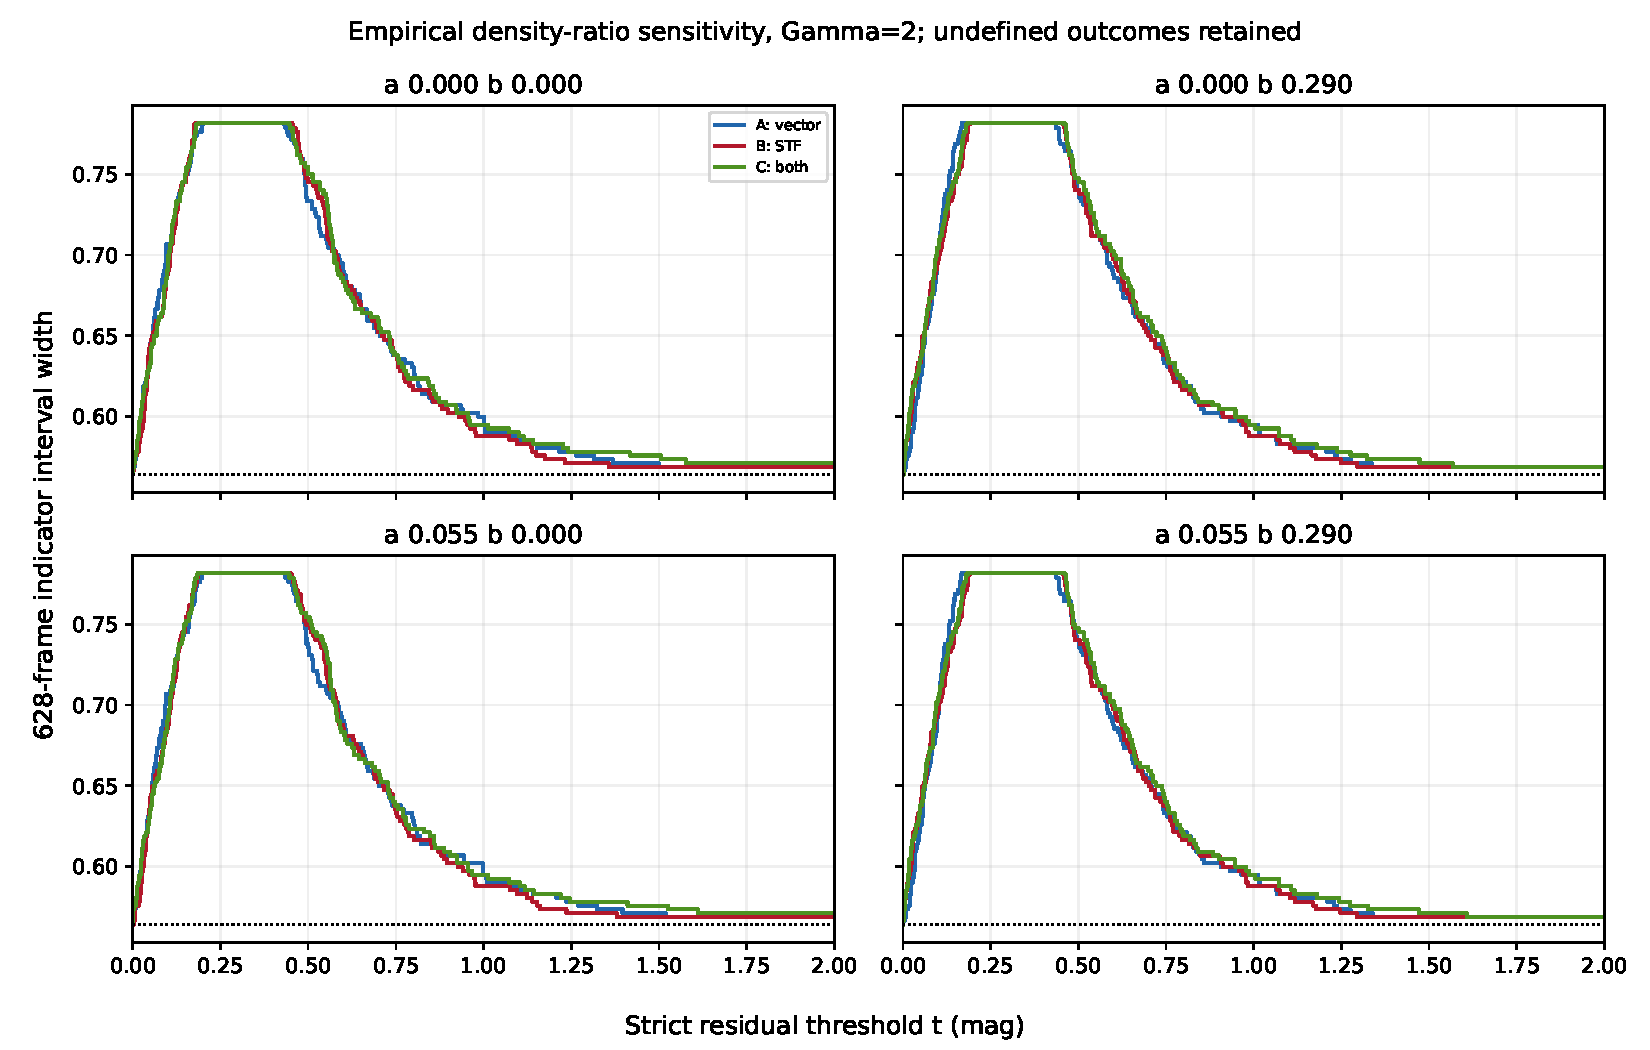
\includegraphics[width=.95\textwidth,height=.75\textheight,keepaspectratio]{figures/selection_bounds.pdf}
\caption{Finite-target sensitivity to weighting and missing event outcomes. The curves retain all twelve model--covariance cases at the declared density-ratio sensitivity level. The missing portion of the 628-target frame remains in every interval hull. At unit density ratio the exact attainable completion set is discrete, with hull width $354/628$. These curves do not estimate a parent selection law or a physical exceedance probability.}
\label{fig:selection}
\end{figure}

\subsection{Auxiliary balance cannot supply absent outcomes}

The retained auxiliary-total calculation provides a source-linked check of transport assumptions. Three cells of the 628-target frame contain no observed distances. Exact nonnegative balance over the full frame is therefore impossible: a positive target mass in any such cell cannot be generated from zero observed support. Deleting those cells defines a different 625-target frame. On this restricted frame, positive weights exist, range from $0.0021333333$ to $0.0064$, and have concentration effective sample size $1/\sum_i p_i^2=271.537086$.

This feasible balancing problem still leaves 351 outcomes missing within supported cells. Finer velocity balancing fails even with signed weights: an observed linear functional vanishes, whereas its target value is nonzero, corresponding to a $2547\,\kms$ discrepancy in the retained within-cell velocity total. Thus the problem is not solved by allowing negative weights or reporting a large concentration effective sample size. The weights constrain auxiliary totals, not the missing response values.

The same positive weights were applied jointly to each retained residual scalar, direction vector, and full STF residual tensor for every model--shape case. This preserves their common atomic dependence. It is a coherent change of finite measure, with no claim that balance proves missing-at-random sampling. In particular, separately choosing weights to improve each scalar summary would no longer describe one transported tensor law.
